% Desenvolvido para o IFSP por: Prof. Dr. David Buzatto (Versão 1.0.2, Data: 31/01/2023)
% Acessado em <https://github.com/davidbuzatto/TemplatesTrabalhosIFSPSBV/tree/master/Template%20Latex%20-%20Apresentacao%20-%20IFSP%20-%20SBV> em 02/02/2023
% Licença Creative Commons CC BY 4.0
% Adaptado para a UFMG por: Dra. Cecilia F. Fiorini (Data: 02/02/2023)

\documentclass[aspectratio=169]{beamer}

% a opção hideSubsectionTitle esconde o título das subseções
\usepackage{estruturaApresentacao}
\usepackage[alf,abnt-emphasize=bf]{abntex2cite}
\usepackage{enumitem}
\newlist{questions}{enumerate}{2}
\setlist[questions,1]{label=P\arabic*.,ref=P\arabic*}
\setlist[questions,2]{label=(\alph*),ref=\thequestionsi(\alph*)}

\begin{document}

\titulo{Trabalho de Aprendizado Descritivo}
% caso não haja, comente a linha abaixo
\subtitulo{Mineração de Dados Urbanos}

\autor{Gruilherme Namen Pimenta}
\orientador{Prof. Dr. Renato Vimieiro}
% caso não haja, comente a linha abaixo
%\coorientador{Prof./Profa. Me./Dr./Dra. Nome Completo}

\curso{Aprendizado Descritivo}

% exemplos
%\curso{Bacharelado em Ciência da Computação}
%\curso{Tecnologia em Sistemas para Internet}
%\curso{Especialização em Desenvolvimento de Aplicações para Dispositivos Móveis}

\local{Belo Horizonte}
\dia{30}
\mes{Julho}
\ano{2024}


% não mexa!

\begin{frame}[plain]
    
    \begin{tikzpicture}[overlay,remember picture]
        \node[left=-0.15cm] at (current page.0){
            
\includegraphics[scale=0.202]{imagens/capa}
        };
    \end{tikzpicture}
    
    \titlepage
    
\end{frame}

\section[Agenda]{}

\begin{frame}
    \frametitle{Outline}
    \begin{columns}[t]
        \begin{column}{.5\textwidth}
            \tableofcontents[sections={1-4}]
        \end{column}
        \begin{column}{.5\textwidth}
            \tableofcontents[sections={5-6}]
        \end{column}
    \end{columns}
\end{frame}

\section{Introdução}

\begin{frame}

    \frametitle{Introdução}

    O processo uso e ocupação do solo dos grandes centros urbanos é alvos de diversos trabalhos da área da sociologia \cite{andrade2020urban, dos2019sapucai, solla2019resistencia}.
    \newline
    \newline
    Com o auxílio da Política de Dados Abertos, os municípios têm divulgados muitas informações, possibilitando grandes avanços no uso de técnicas de aprendizado de máquina para auxiliar as políticas sociais e econômicas.
\end{frame}

\subsection{Questionamentos}
\begin{frame}

    \frametitle{Questionamentos}

    \begin{questions}
        \item Quais os algoritmos de mineração de dados são úteis para descrever uma base de dados urbanos?
        \item Quais informações eles podem gerar?
        \item Qual é a melhor sequência de algoritmos para descrever os dados e formar a arquitetura de dutos?
\end{questions}
\end{frame}

\subsection{Objetivos}
\begin{frame}

    \frametitle{Objetivos}

    \begin{itemize}
    
        \item Objetivo Geral
            \begin{itemize}
                \item Adaptar a arquitetura de dutos e filtros de descoberta de conhecimento em banco de dados \cite{nwagu2017knowledge}, utilizando um conjunto mínimo de algoritmos de mineração de dados.
                \item Gerar conhecimento aplicado ao uso e ocupação do solo de áreas urbanas.
            \end{itemize}
            
        \item Objetivos Específicos
            \begin{itemize}
                \item Coleta, limpeza e armazenamento de dados;
                \item Pré processamento de dados;
                \item Definir metodologia para escolha dos algoritmos;
                \item Executar os algoritmos;
                \item Apresentar o conhecimento gerado;
                \item Responder as perguntas de pesquisa;
            \end{itemize}
            
    \end{itemize}

\end{frame}
\section{Processamentos dos Dados}


\subsection{Coleta}

\begin{frame}

    \frametitle{Coleta dos Dados}

    Os dados forma coletados no Portal de Dados Abertos da Prefeitura de Belo Horizonte, https://ckan.pbh.gov.br/.
    \newline
    \newline
    Os dados são referentes às guias de IPTU da data de 03/06/2024.
    \newline
    \newline
    As informações são da Secretaria Municipal de Fazenda.

\end{frame}


\begin{frame}

    \frametitle{Descrição dos Dados}
    Os dados contém várias informações dos imóveis, tais como endereço, área do terreno, área construída, geometria do terreno e outras. A descrição completa encontra-se no Portal de dados abertos
\end{frame}


\subsection{As Regionais de Belo Horizonte}

\begin{frame}

    \frametitle{Mapas das Regionais}
    \begin{columns}[t]
        \begin{column}{7cm}
            \begin{figure}[!htbp]
                \centering
       	    %\caption{Área das Regionais de Belo Horizonte}
       	    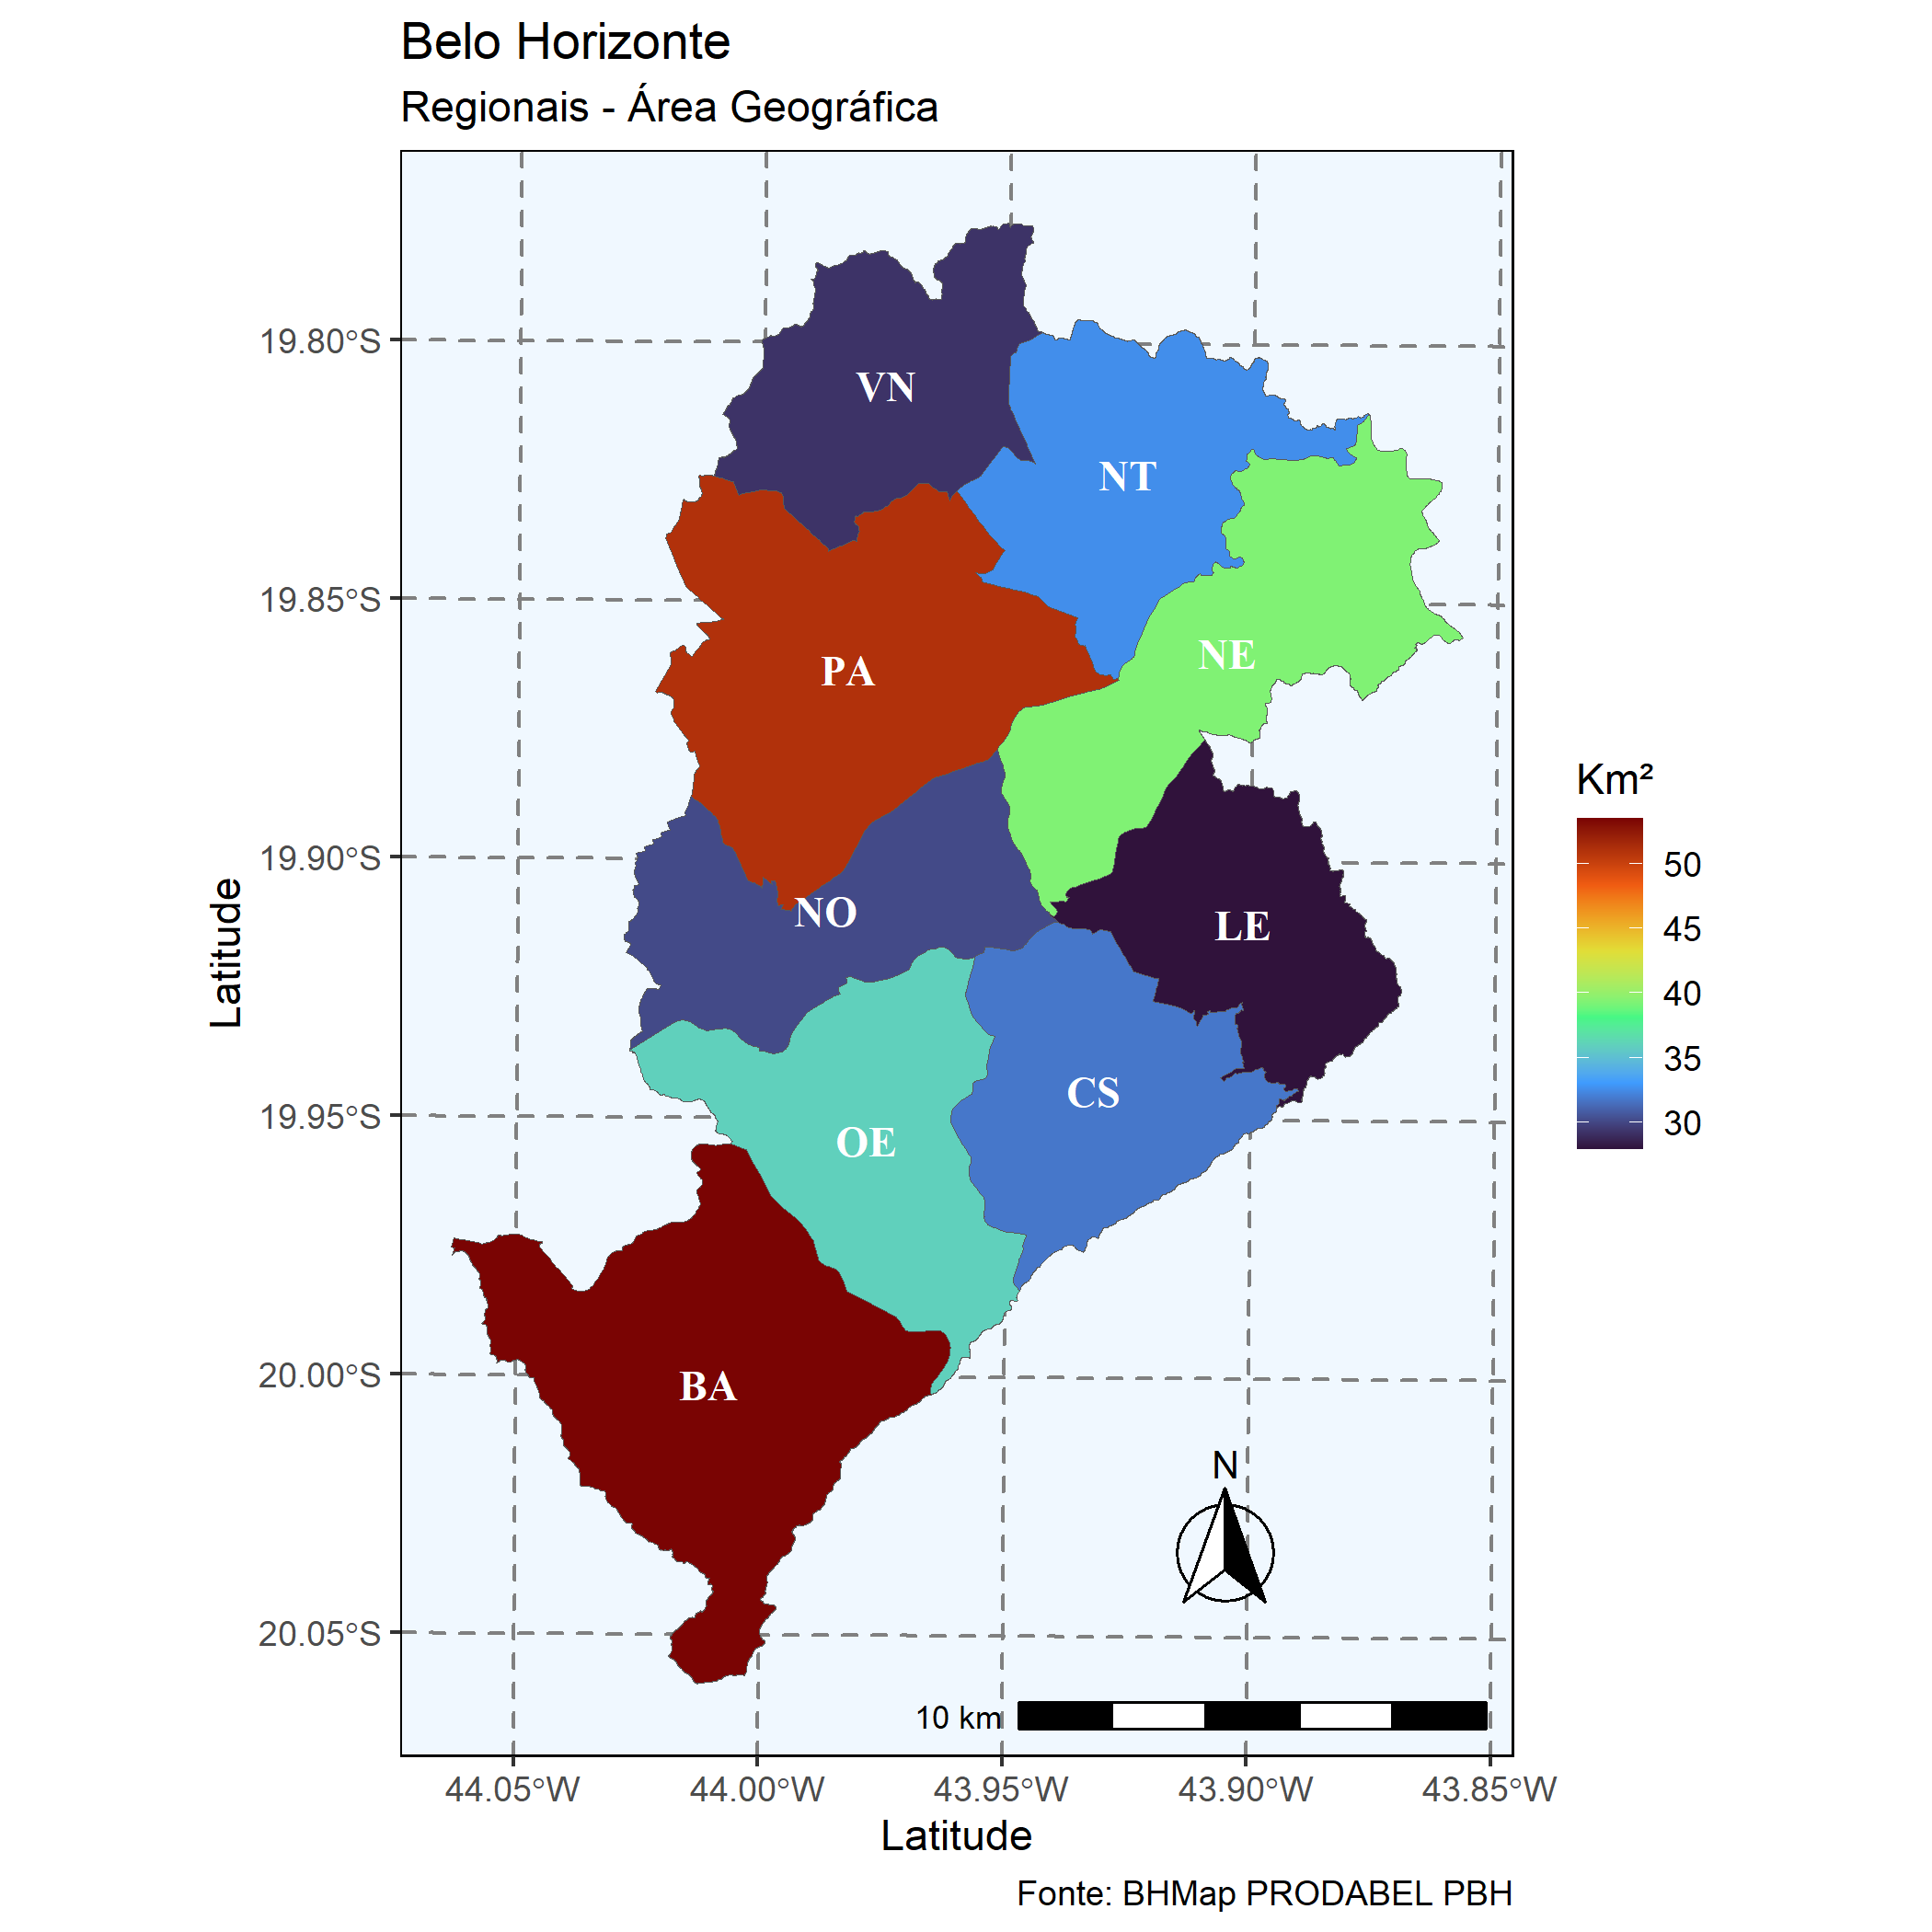
\includegraphics[scale=0.30]{imagens/area.png}
            \end{figure}
        \end{column}
        \begin{column}{7cm}
            \begin{figure}[!htbp]
                \centering
       	    %\caption{População das Regionais de Belo Horizonte}
       	    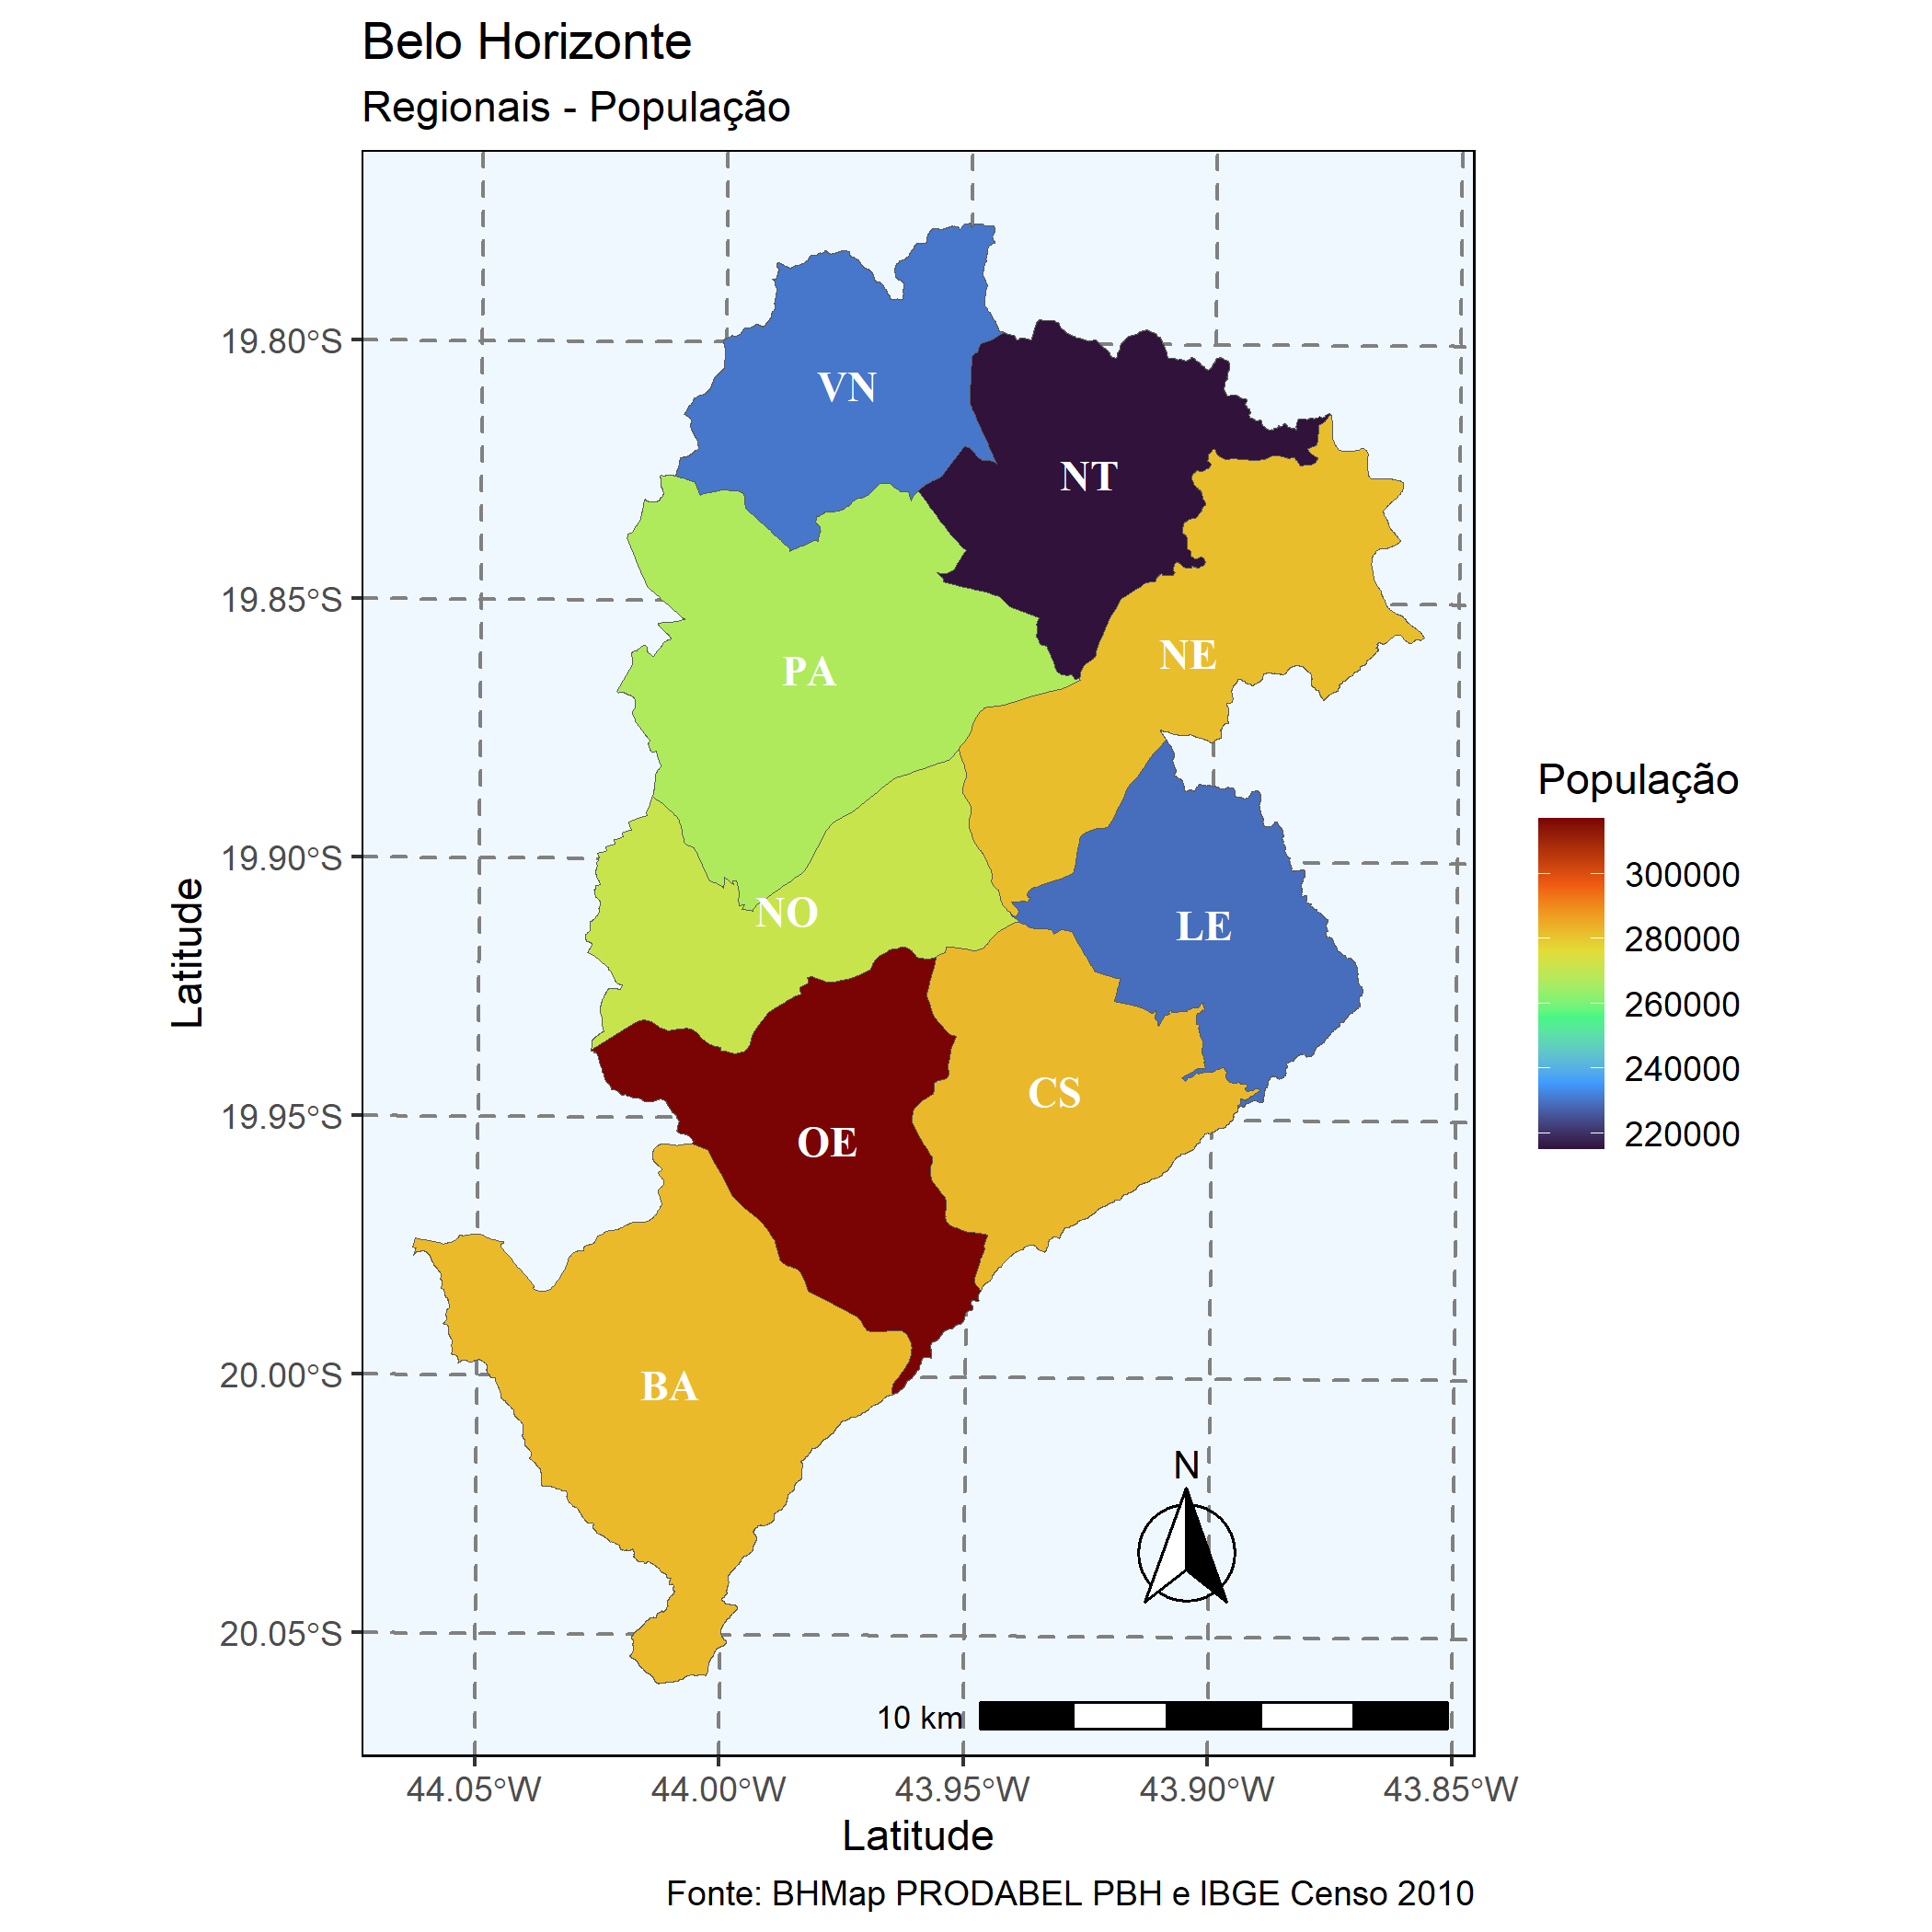
\includegraphics[scale=0.30]{imagens/populacao.png}
            \end{figure}
        \end{column}
    \end{columns}
\end{frame}


\begin{frame}

    \frametitle{Mapas das Regionais}

    \begin{columns}[t]
        \begin{column}{7cm}
            \begin{figure}[!htbp]
                \centering
       	    %\caption{Área das Regionais de Belo Horizonte}
       	    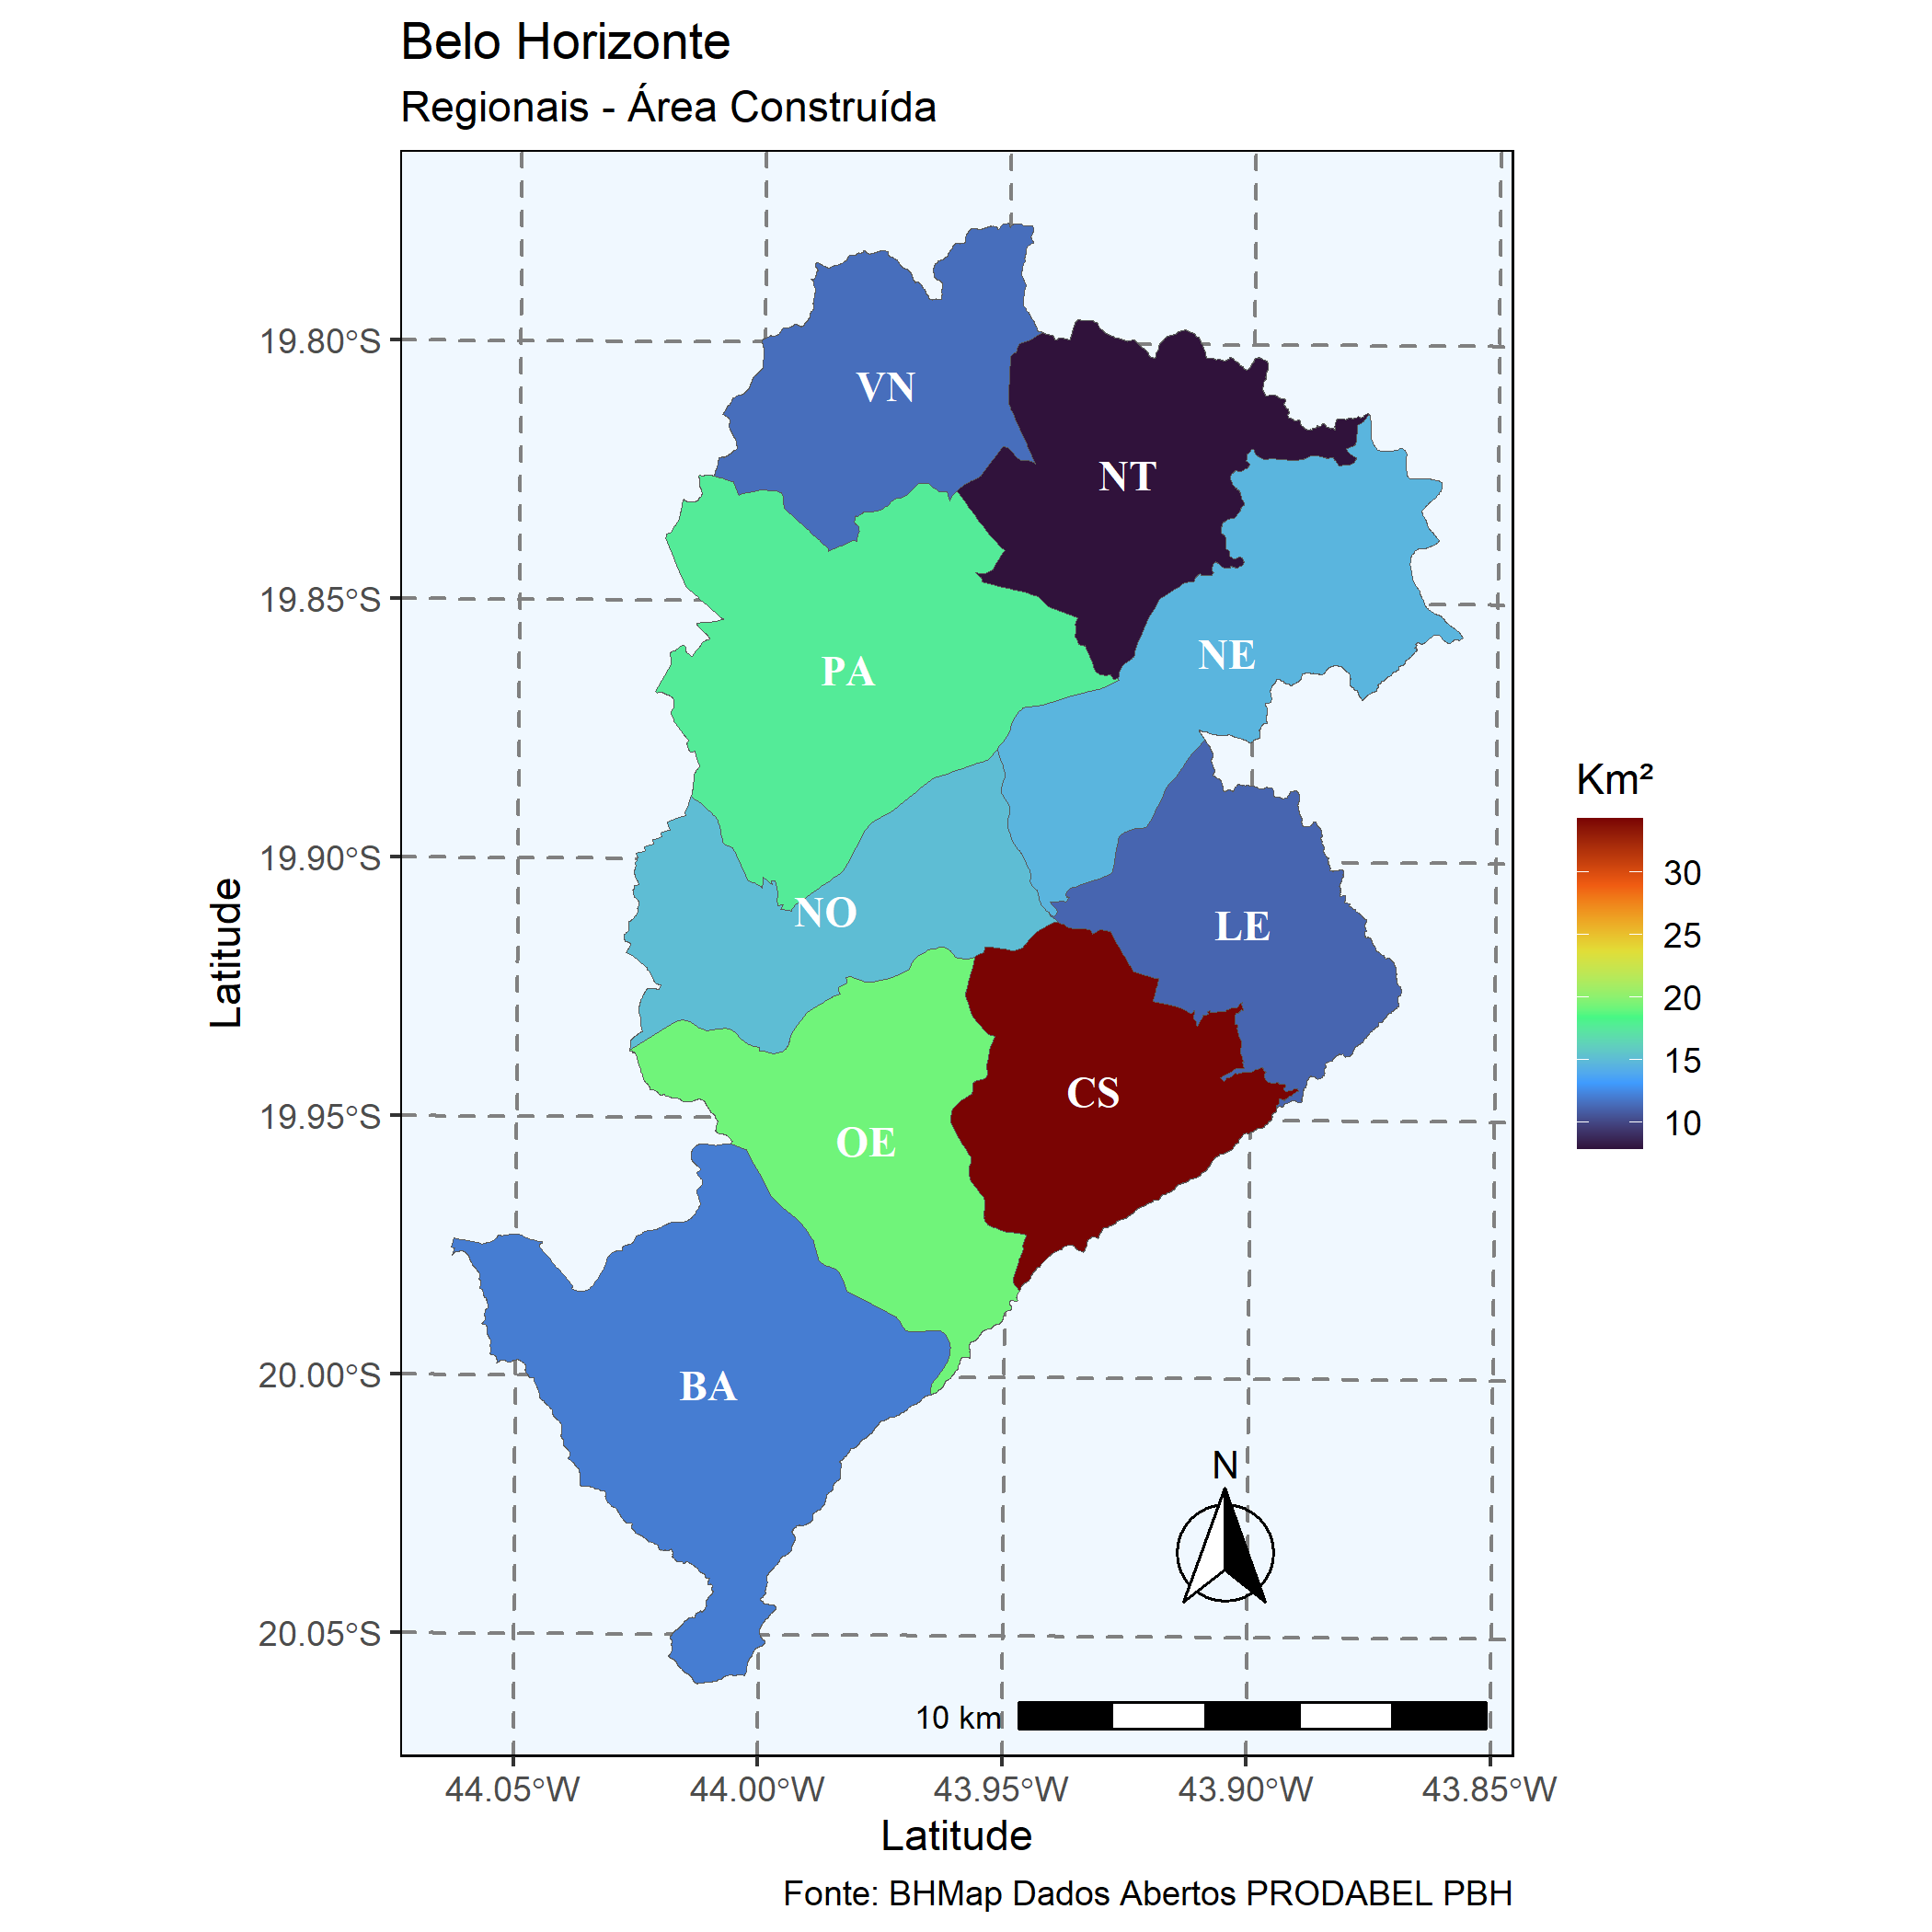
\includegraphics[scale=0.30]{imagens/area_construida.png}
            \end{figure}
        \end{column}
        \begin{column}{7cm}
            \begin{figure}[!htbp]
                \centering
       	    %\caption{População das Regionais de Belo Horizonte}
       	    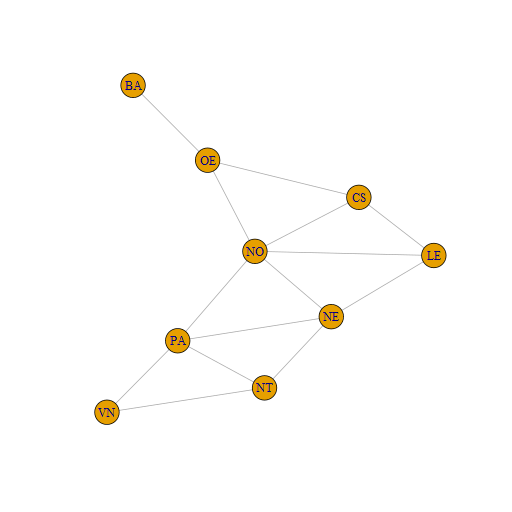
\includegraphics[scale=0.35]{imagens/grafo.png}
            \end{figure}
        \end{column}
    \end{columns}
\end{frame}


\subsection{Características}

\begin{frame}

    \frametitle{Coleta de Lixo}
    \begin{figure}[!htbp]
                \centering
       	    %\caption{População das Regionais de Belo Horizonte}
       	    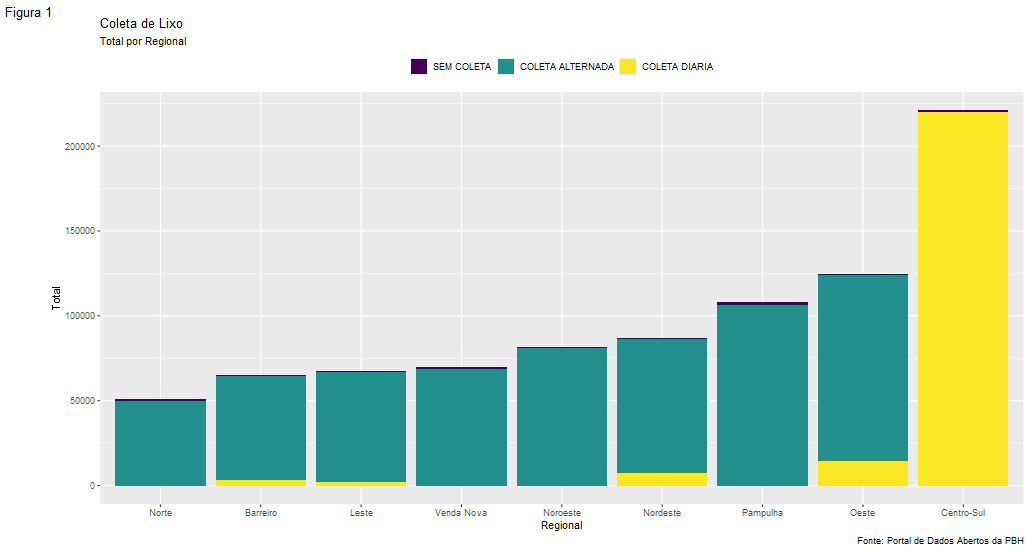
\includegraphics[scale=0.35]{imagens/coleta.png}
            \end{figure}

\end{frame}
\begin{frame}

    \frametitle{Perfil}
    \begin{figure}[!htbp]
                \centering
       	    %\caption{População das Regionais de Belo Horizonte}
       	    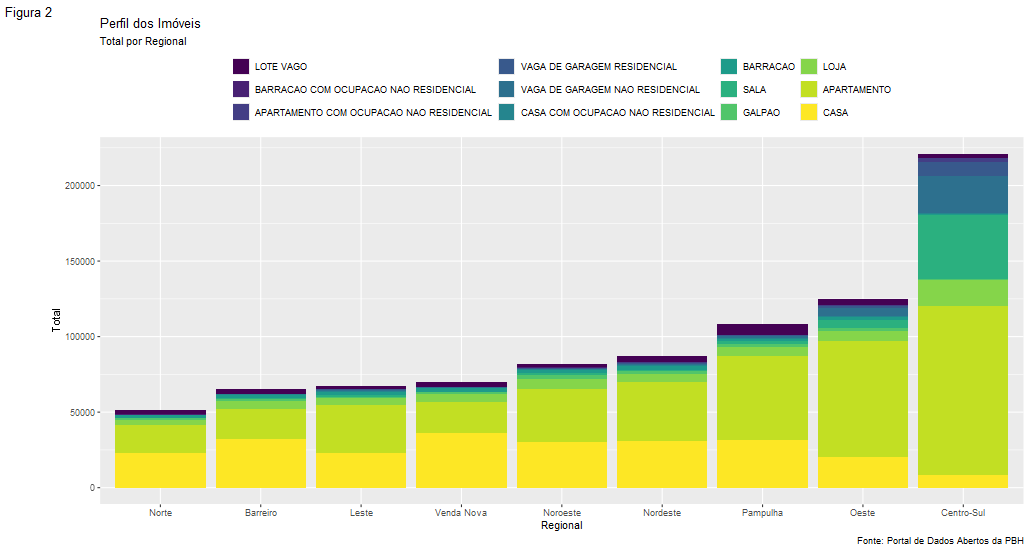
\includegraphics[scale=0.35]{imagens/perfil.png}
            \end{figure}

\end{frame}

\begin{frame}

    \frametitle{Ocupação}
    \begin{figure}[!htbp]
                \centering
       	    %\caption{População das Regionais de Belo Horizonte}
       	    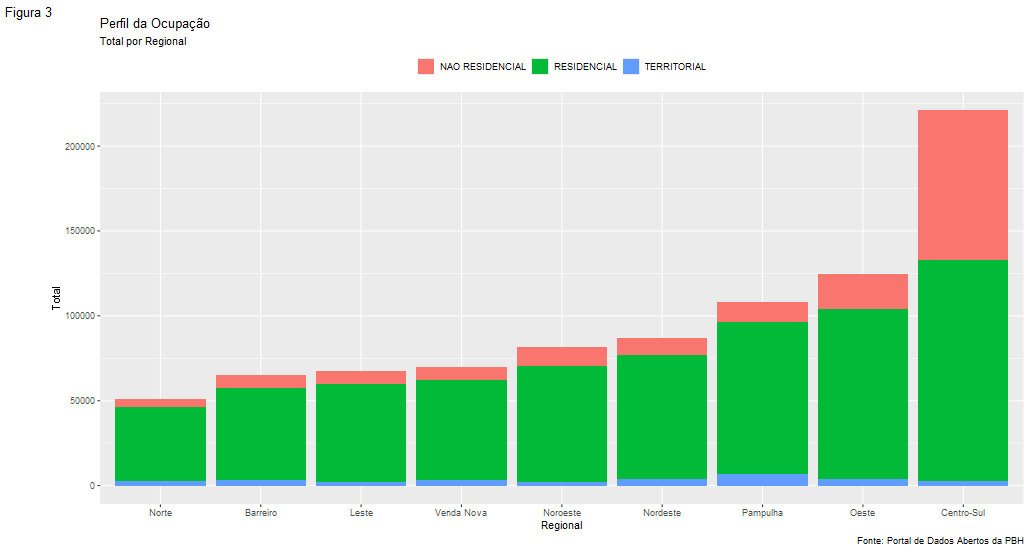
\includegraphics[scale=0.35]{imagens/ocupacao.png}
            \end{figure}

\end{frame}

\begin{frame}

    \frametitle{Qualidade do Acabamento}
    \begin{figure}[!htbp]
                \centering
       	    %\caption{População das Regionais de Belo Horizonte}
       	    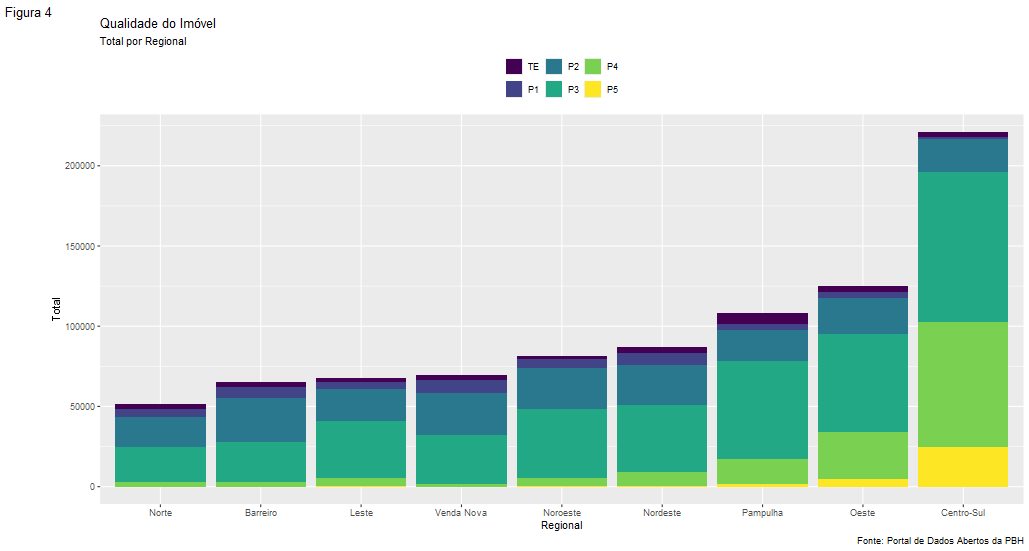
\includegraphics[scale=0.35]{imagens/acabamento.png}
            \end{figure}

\end{frame}
\section{Metodologia}


\begin{frame}

    \frametitle{Metodologia}

    Para a escolha dos algoritmos foi utilizado o Princípio da Descrição de Comprimento Mínimo (DCM) da mesma forma que foi utilizado na tese de Proença \cite{proencca2021robust}.
    \newline
    \newline
    Para guiar o processo de criação da arquitetura foi utilizado a metodologia \textit{Goal Question Metric (GQM)} \cite{caldiera1994goal}, metodologia muito utilizada no campo da Engenharia de Software \cite{sommerville2011software}.

\end{frame}

\subsection{Arquitetura de Dutos e Filtros}
\begin{frame}

    \frametitle{Estrutura da Arquitetura de Dutos e Filtros}

    \begin{figure}[!htbp]
                \centering
       	    \caption{Exemplo de um pipeline}
       	    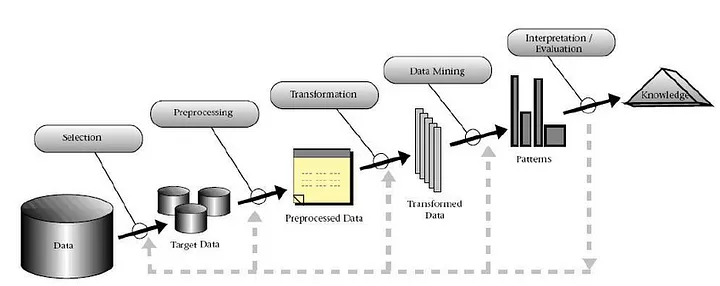
\includegraphics[scale=0.65]{imagens/pipeline.png}
            \end{figure}

\end{frame}


\begin{frame}
    \frametitle{Definição das Fases}
     \begin{itemize}
        \item Pré-Processamento
            \begin{itemize}
                \item Uso da ferramenta \textbf{GritBot} da RuleQuest Research para detectar anomalias (\textit{outliers}).
            \end{itemize}
            
        \item Transformação
            \begin{itemize}
                \item \textbf{\textit{Outlier}}: Maiores áreas construídas;
                \item \textbf{Item}: Tipo Construtivo X Padrão de Acabamento X \textit{Outlier};
                \item \textbf{Transações}: agrupamento por CEP;
                \item \textbf{Utilidade}: área construída;
                \item \textbf{Utilidade Negativa}: área do terreno vago;
            \end{itemize}
    \end{itemize}
\end{frame}

\begin{frame}
    \frametitle{Mineração de Dados}
     \begin{itemize}
        \item Algoritmos
            \begin{itemize}
                \item \textbf{FPClose} - Algoritmo eficiente para obter os itemsets fechados mais frequêntes;
                \item \textbf{OpusMiner} - Algorigmo para obter os itemsets estatisticamente relevantes;
                \item \textbf{FHM Freq} - Algoritmo para obter os itemsets de maior utilidade e suporte.
                \item \textbf{FHN} - Algoritmo para processar itemsets de utilidade negativa;
                \item \textbf{Cortana} - \textit{Software} para processar subgrupos de interesse.
            \end{itemize}
    \end{itemize}
\end{frame}
\section{Resultados}

\subsection{Itemsets Frequênts}
\begin{frame}

    \frametitle{Resultados}

    \begin{itemize}
    
        \item Regionais Distantes do Centro
            \begin{itemize}
                \item Caracterizadas pela maioria de casas de padrões de acabamento entre um e três e lotes vagos;
                \item A Pampulha se destaca por ter casas de padrão 4 e não apresentar casas com acabamento padrão 1.
            \end{itemize}
            
        \item Regionais Vizinhas ao Centro
            \begin{itemize}
                \item Regionais Oeste e Nordeste predominam casas com padrão igual às regionais mais distantes;
                \item Leste e Noroeste possuem um padrão misto de casas, barracões, comércio local e lotes vagos, com padrões variando do 1 ao 3.
            \end{itemize}
        \item Regional Centro Sul
            \begin{itemize}
                \item Todos os itemset apresentaram apenas um item, com padrões variando do 3 ao 4;
                \item Indicação de segmentação ordenada do espaço.
            \end{itemize}
            
    \end{itemize}

\end{frame}

\subsection{Itemsets estatisticamente relevantes}
\begin{frame}
 \frametitle{Resultados}
   \begin{itemize}
    
        \item Indicou a forte presença conjugada de salas comerciais de alto padrão de acabamento com a existência de vagas de garagem;
        \item Indicou adaptação de imóveis de moradia para a finalidade comercial conjugados com imóveis comerciais;
        \item Indicou a presença conjugadas de imóveis de maior área construída próximos a imóveis padrão de mesmo acabamento ou superiores;
        \item A regional Centro-Sul possui uma grande quantidade de salas de alto padrão conjugadas com vagas de garagem.
    \end{itemize}

\end{frame}

\subsection{Utilidade em m² construídos}
\begin{frame}

    \begin{itemize}
    
        \item Presença de comércio local nas regionais Barreiro, Nordeste, Norte e Venda Nova;
        \item Regional Oeste apresenta uma grande quantidade de apartamentos com acabamento 3, totalizando mais de 4 km² construídos;
	\item A regional Noroeste possui uma grande área construída destinada a galpões;
        \item A regional Centro-Sul possui muitos centros comerciais com muita área construída.
    \end{itemize}
\end{frame}

\begin{frame}

    \begin{figure}[!htbp]
                \centering
       	    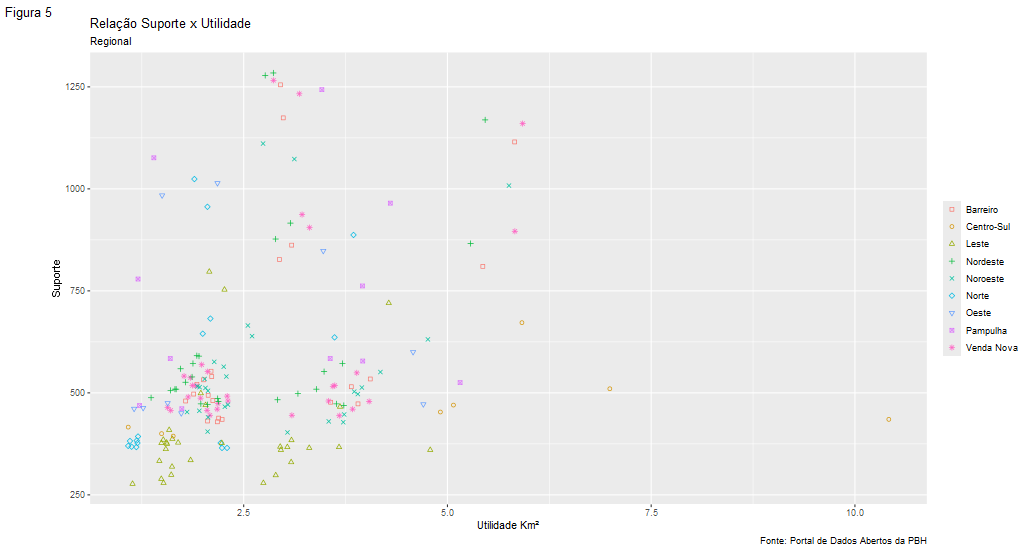
\includegraphics[scale=0.35]{imagens/utilidade_suporte.png}
            \end{figure}
\end{frame}

\subsection{Utilidade negativa m²}
\begin{frame}

    \begin{itemize}
    
        \item As regionais Pampulha e Norte tiveram um impacto negativo em lotes vagos, indicando áreas vagas proximas a terrenos com construção.
    \end{itemize}
\end{frame}

\subsection{Descoberta de Subgrupo - Alvo Padrão de Acabamento P5}
\begin{frame}

    \begin{figure}[!htbp]
                \centering
       	    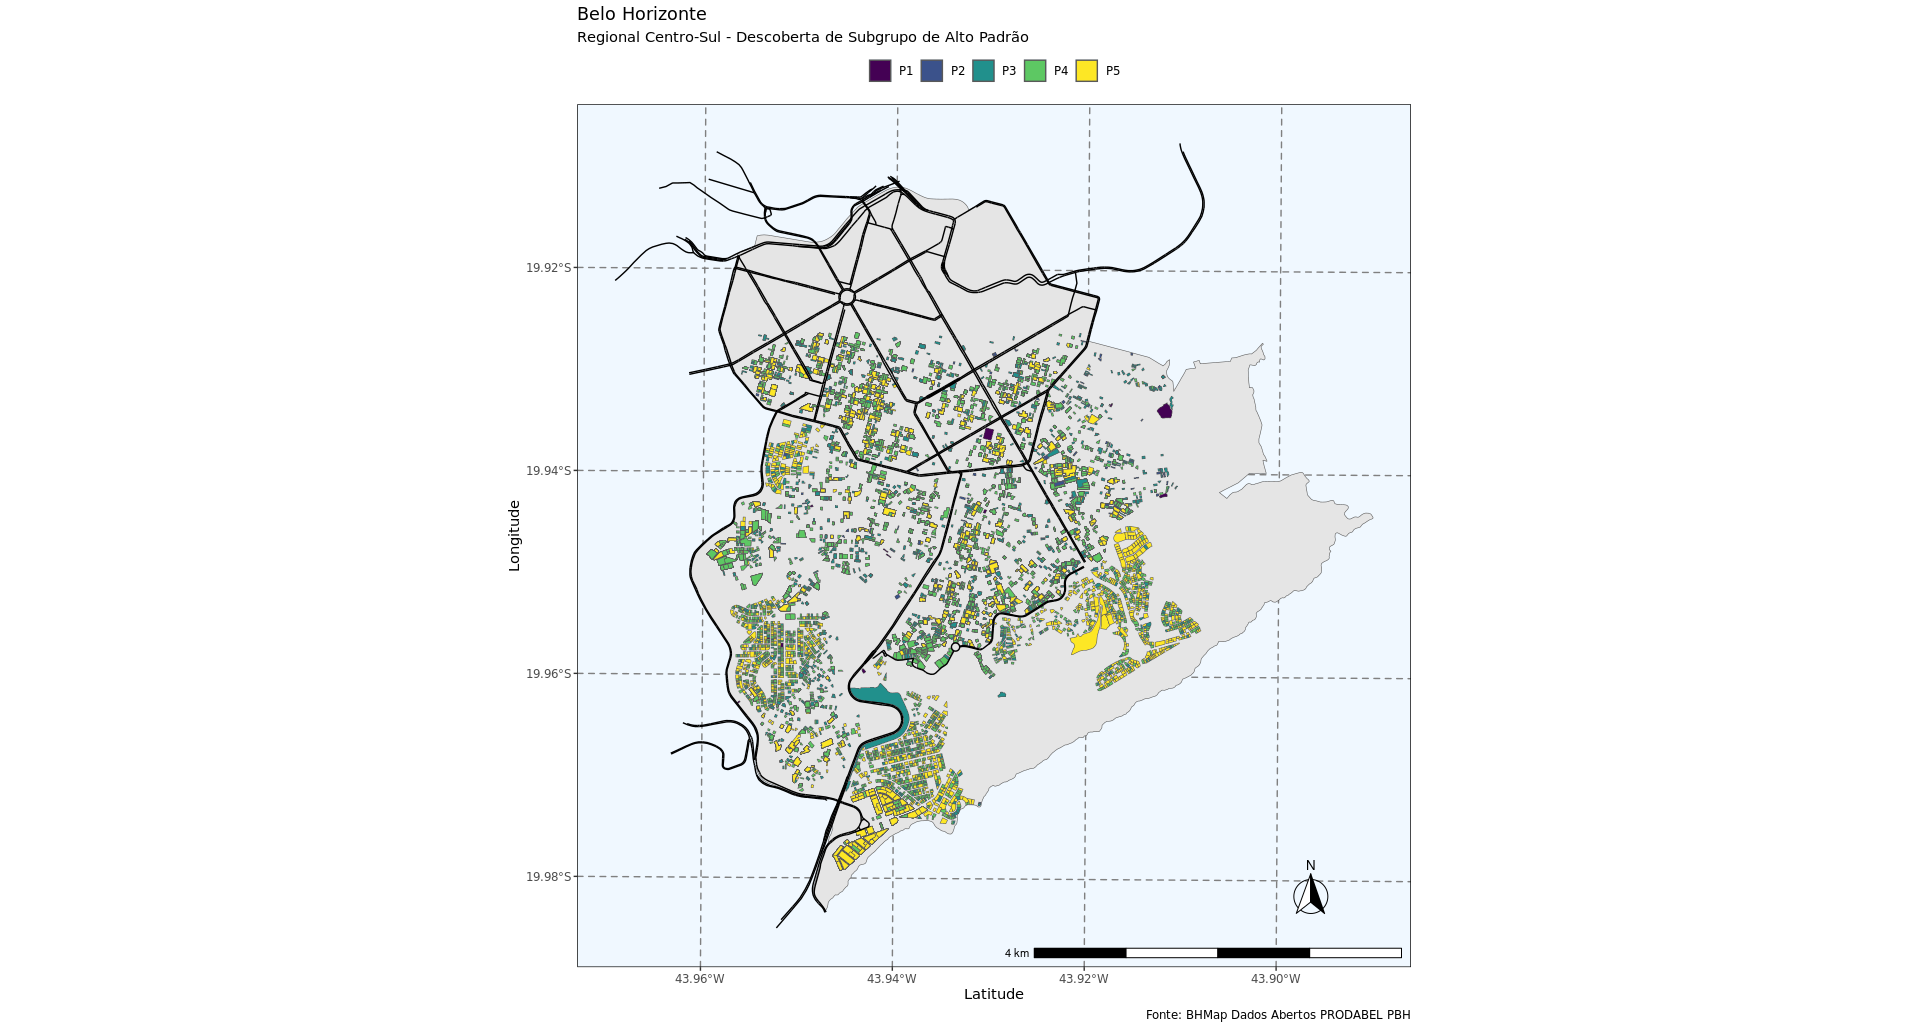
\includegraphics[scale=0.26]{imagens/cortana3.png}
            \end{figure}
\end{frame}

\subsection{Descoberta de Subgrupo - Alvo Tipo Construtivo Apartamento}
\begin{frame}

    \begin{figure}[!htbp]
                \centering
       	    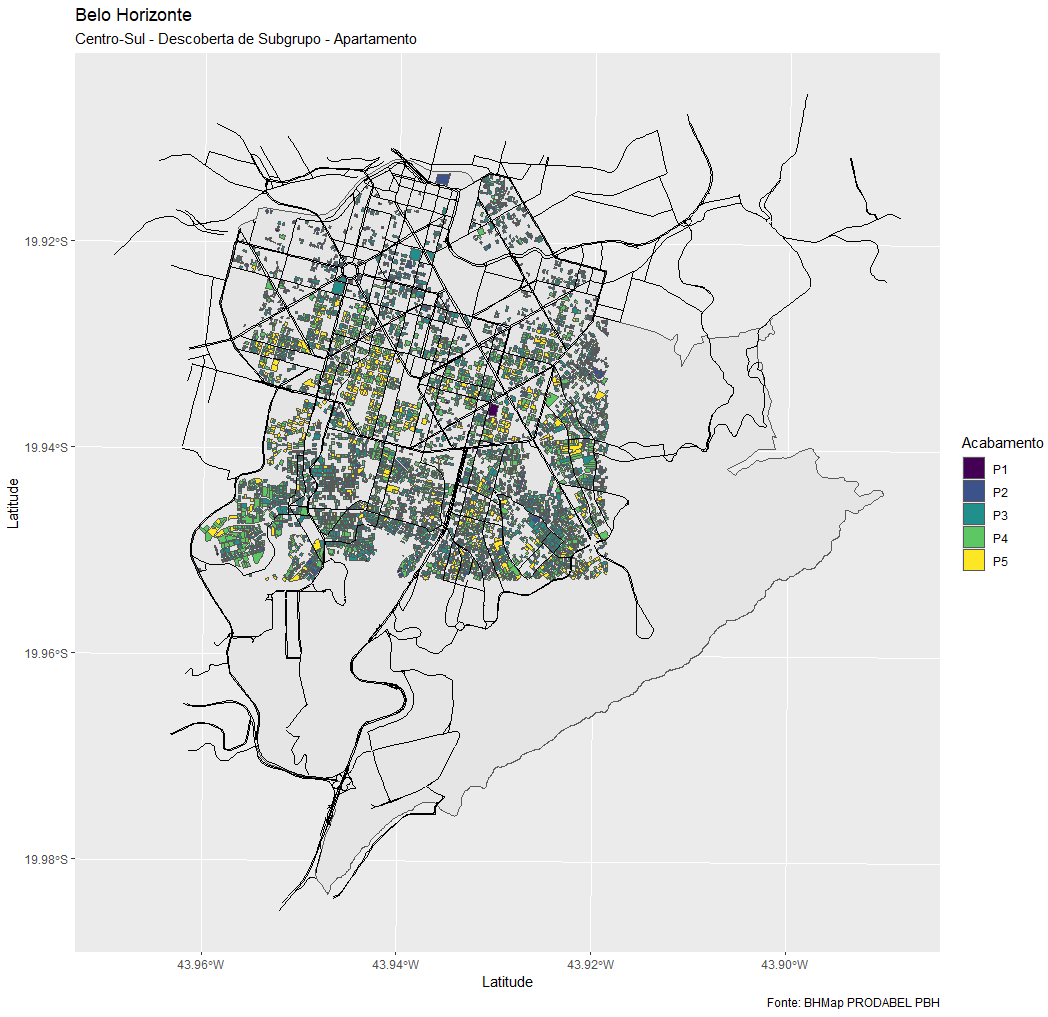
\includegraphics[scale=0.26]{imagens/cortana-ap.png}
            \end{figure}
\end{frame}

\subsection{Descoberta de Subgrupo - Gentrificação}
\begin{frame}

	\begin{table}[]
		\begin{tabular}{|l|l|}
			\hline
			\textbf{Zona Homogenia} & \textbf{Núcleos Familiáres}\\
			\hline
			\hline
			CS407 & 10 \\
			\hline
			CS313 & 12 \\
			\hline
			CS210, CS212 & 13 \\
			\hline
			CS411 & 23 \\
			\hline
		\end{tabular}
	\end{table}
\end{frame}
\subsection{Gentrificação}
\begin{frame}

    \begin{figure}[!htbp]
                \centering
       	    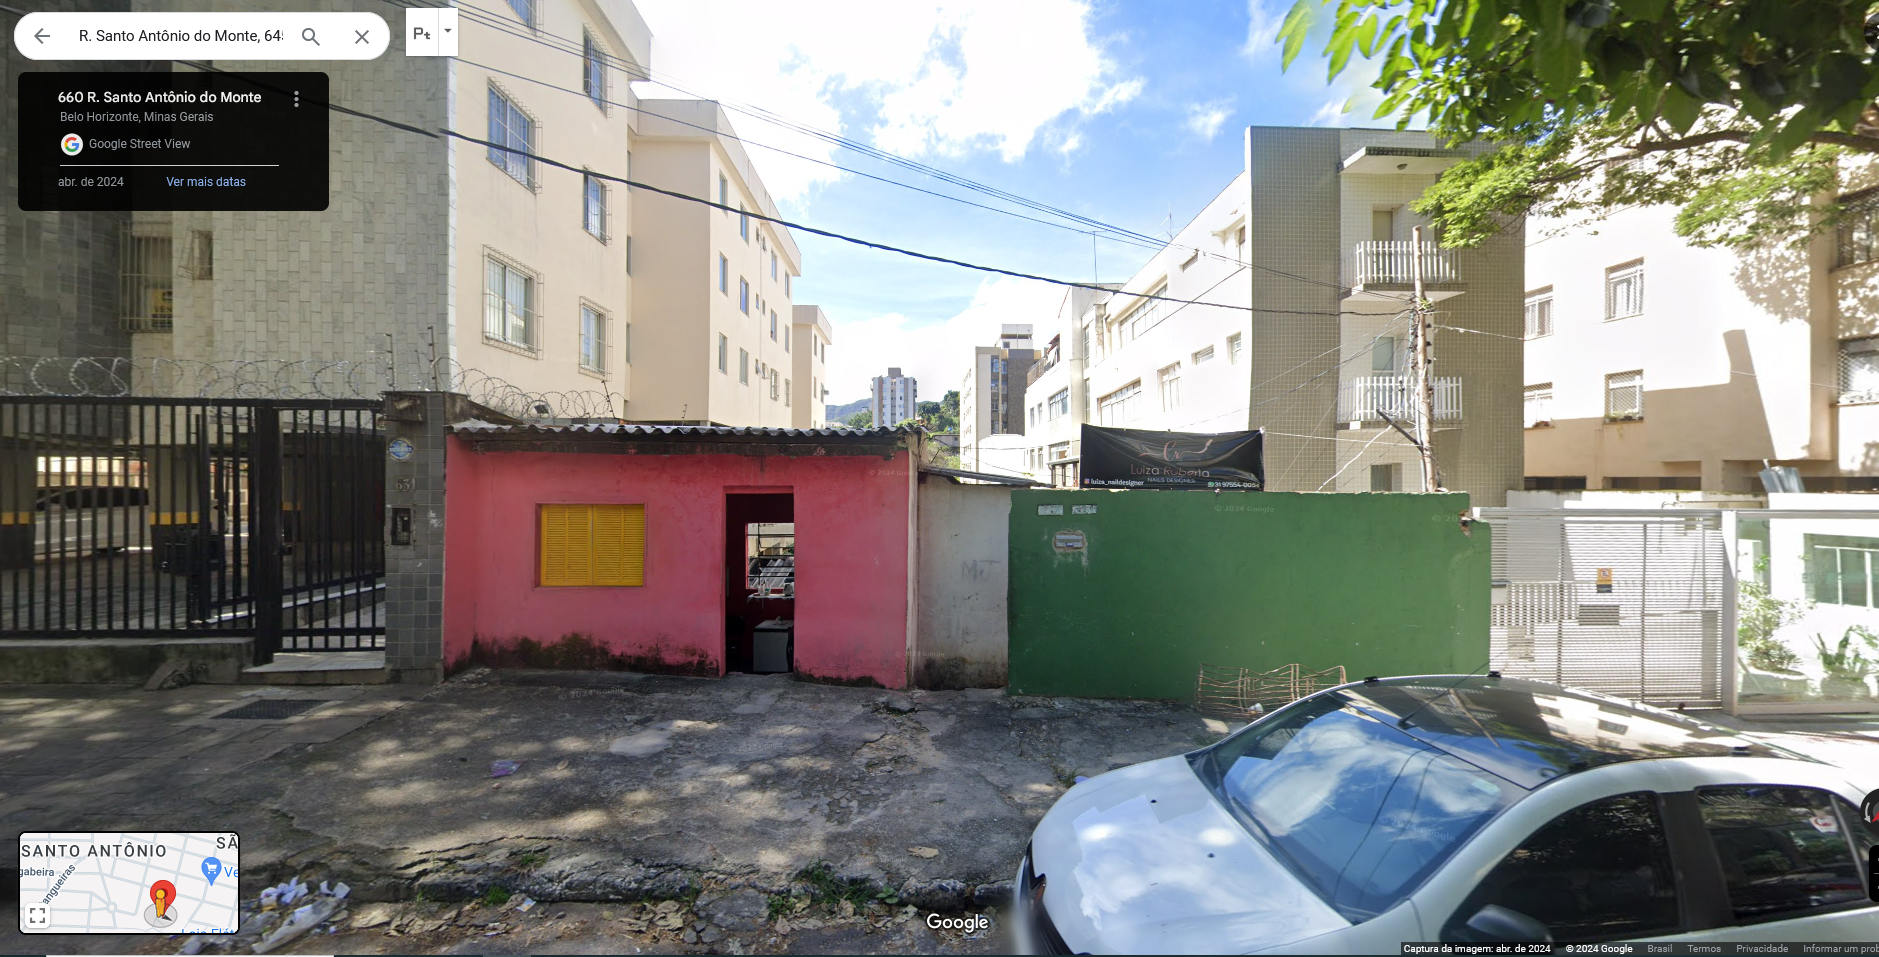
\includegraphics[scale=0.26]{imagens/gentrificacao.png}
            \end{figure}
\end{frame}



\section{Conclusão e Trabalhos Futuros}


\begin{frame}

    \frametitle{Respostas}

    \begin{questions}
        \item Os algoritmos de mineração de dados mais úteis para descrever uma base de dados foram: FPMax, OpusMiner, FHM Freq, FHN e Descoberta de Subgrupo. Esta sequência de algoritmos descrevem os dados de forma mais genérica à mais específica.
        \item Eles conseguem, em sequência, gerarem um conjunto de informações mais genéricas até as mais específicas.
        \item A melhor sequência de execução dos algoritmos foi a apresentada no trabalho, a grande descoberta do trabalho foi que para utilizar o algoritmo de descoberta de subgrupos de forma mais eficiênte, a melhor forma, é compreender a base de dados para segmentar muito bem os registros que serão processados.
\end{questions}

\end{frame}


\begin{frame}

    \frametitle{Conclusão}

    O trabalho demonstrou a eficacia de uma arquitetura de dutos e filtros com algoritmos de mineração de dados para descrever o espaço urbano de Belo Horizonte de forma compacta, revelando padroes e tendências no uso e ocupação do solo a partir de dados imobiliarios.

\end{frame}


\begin{frame}

    \frametitle{Trabalhos Futuros}

	Destaca-se a incorporação de dados espaço-temporais para análise de séries históricas.
	\newline
	\newline
	A integração com outras fontes de dados, como redes sociais e imagens de satélite.
	\newline
	\newline
	E uso de outras técnicas de mineração de dados como a mineração de dados de mesma localidade, para evitar a segmentação por regionais.
\end{frame}


\begin{frame}
    \begin{center}
        \Huge{OBRIGADO!}
    \end{center}
\end{frame}



% exemplos de construções em LaTeX
% comente a linha abaixo para gerar a versão final
%\section{Exemplos}


\begin{frame}

    \frametitle{Título do Slide}

    Texto corrido normal .
    
    \begin{huge}
        Texto com fonte gigante.
    \end{huge}
    
    \begin{LARGE}
        Texto com fonte GRANDE.
    \end{LARGE}
        
    \begin{Large}
        Texto com fonte Grande.
    \end{Large}
    
    \begin{large}
        Texto com fonte grande.
    \end{large}
    
    \begin{normalsize}
        Texto com fonte normal.
    \end{normalsize}
        
    \begin{small}
        Texto com fonte pequena.
    \end{small}
        
    \begin{footnotesize}
        Texto com fonte do tamanho de nota de rosapé.
    \end{footnotesize}
    
    \begin{scriptsize}
        Texto com fonte do tamanho de letra manuscrita.
    \end{scriptsize}
        
    \begin{tiny}
        Texto com fonte minúscula.
    \end{tiny}        

\end{frame}


\begin{frame}

    \frametitle{Slide com Duas Colunas}
    
    \begin{columns}[t]
    
        \begin{column}{7cm}

            Conteúdo da coluna 1.

        \end{column}

        \begin{column}{7cm}

            Conteúdo da coluna 2.

        \end{column}

    \end{columns}
        
\end{frame}


\begin{frame}

    \frametitle{Slide com Blocos}
    
    Exemplos de blocos de texto. Cuidado para não abusar no uso, evitando que os slides fiquem muito ``carregados''.
    
    \begin{block}{Observação}
        Caixa de texto padrão.
    \end{block}
    
    \begin{exampleblock}{Exemplo}
        Caixa de texto de exemplo.
    \end{exampleblock}
        
    \begin{alertblock}{Importante}
        Caixa de texto de alerta.
    \end{alertblock}
    
    \definecolor{corFundoTitulo}{RGB}{95, 40, 113}
    \definecolor{corTextoTitulo}{RGB}{255, 255, 255}
    \definecolor{corFundoConteudo}{RGB}{114, 140, 166}
    \definecolor{corTextoConteudo}{RGB}{0, 0, 0}
    \begin{bloco}{Bloco com cores customizadas}{bg=corFundoConteudo,fg=corTextoConteudo}{bg=corFundoTitulo,fg=corTextoTitulo}
        Conteúdo
    \end{bloco}
         
\end{frame}


\begin{frame}

    \frametitle{Slide com Desenhos Usando Tikz}
    
    Desenhando formas...
    
    \begin{center}
        
\begin{tikzpicture}[scale=1.0]
            \draw[blue, very thick] (0,0) rectangle (3,2);
            \draw[orange, ultra thick] (4,0) -- (6,0) -- (5.7,2) -- cycle;
        \end{tikzpicture}
    \end{center}
         
\end{frame}


\begin{frame}

    \frametitle{Slide com Desenhos Usando Tikz}
    
    Uma Máquina de Turing que realiza a operação subtração própria.
    
    \begin{center}
        \begin{tikzpicture} [scale=0.75, every node/.style={transform shape}, node distance = 3cm, on grid]

            \node (q0) [state,
                initial,
                initial text=Início
            ] {$q_0$};
            \node (q1) [state, right = of q0] {$q_1$};
            \node (q2) [state, right = of q1] {$q_2$};
            \node (q3) [state, right = of q2] {$q_3$};
            \node (q5) [state, below = of q0] {$q_5$};
            \node (q6) [state, below = of q1] {$q_6$};
            \node (q4) [state, below = of q2] {$q_4$};
                        
            \path [-stealth]
                (q0) edge node[above] {$0/B\rightarrow$} (q1)
                (q1) edge [loop below] node {$0/0\rightarrow$} ()
                (q1) edge node[above] {$1/1\rightarrow$} (q2)
                (q2) edge [loop below] node[right] {$1/1\rightarrow$} ()
                (q2) edge node[above] {$0/1\leftarrow$} (q3)
                
                (q3) edge [loop below] node {$
                    \begin{aligned}
                      0 &/ 0\leftarrow\\[-0.7ex]
                      1 &/ 1\leftarrow
                    \end{aligned}$} ()
                
                (q3) edge [bend right] node[above] {$B/B\rightarrow$} (q0)
                
                (q0) edge [bend right] node[left] {$1/B\rightarrow$} (q5)
                (q2) edge [bend right] node[left] {$B/B\leftarrow$} (q4)
                
                (q5) edge [loop below] node {$
                    \begin{aligned}
                      0 &/ B\rightarrow\\[-0.7ex]
                      1 &/ B\rightarrow
                    \end{aligned}$} ()
                                    
                (q5) edge node[above] {$B/B\rightarrow$} (q6)
                
                (q4) edge [loop below] node {$
                    \begin{aligned}
                      0 &/ 0\leftarrow\\[-0.7ex]
                      1 &/ B\leftarrow
                    \end{aligned}$} ()
                                    
                (q4) edge node[above] {$B/0\rightarrow$} (q6);
        
        \end{tikzpicture}
    \end{center}
         
\end{frame}


\begin{frame}

    \frametitle{Slide com Figura}
    
    \begin{figure}[!htbp]
       	\centering
       	\caption{Exemplo de figura (caption é opcional)}
       	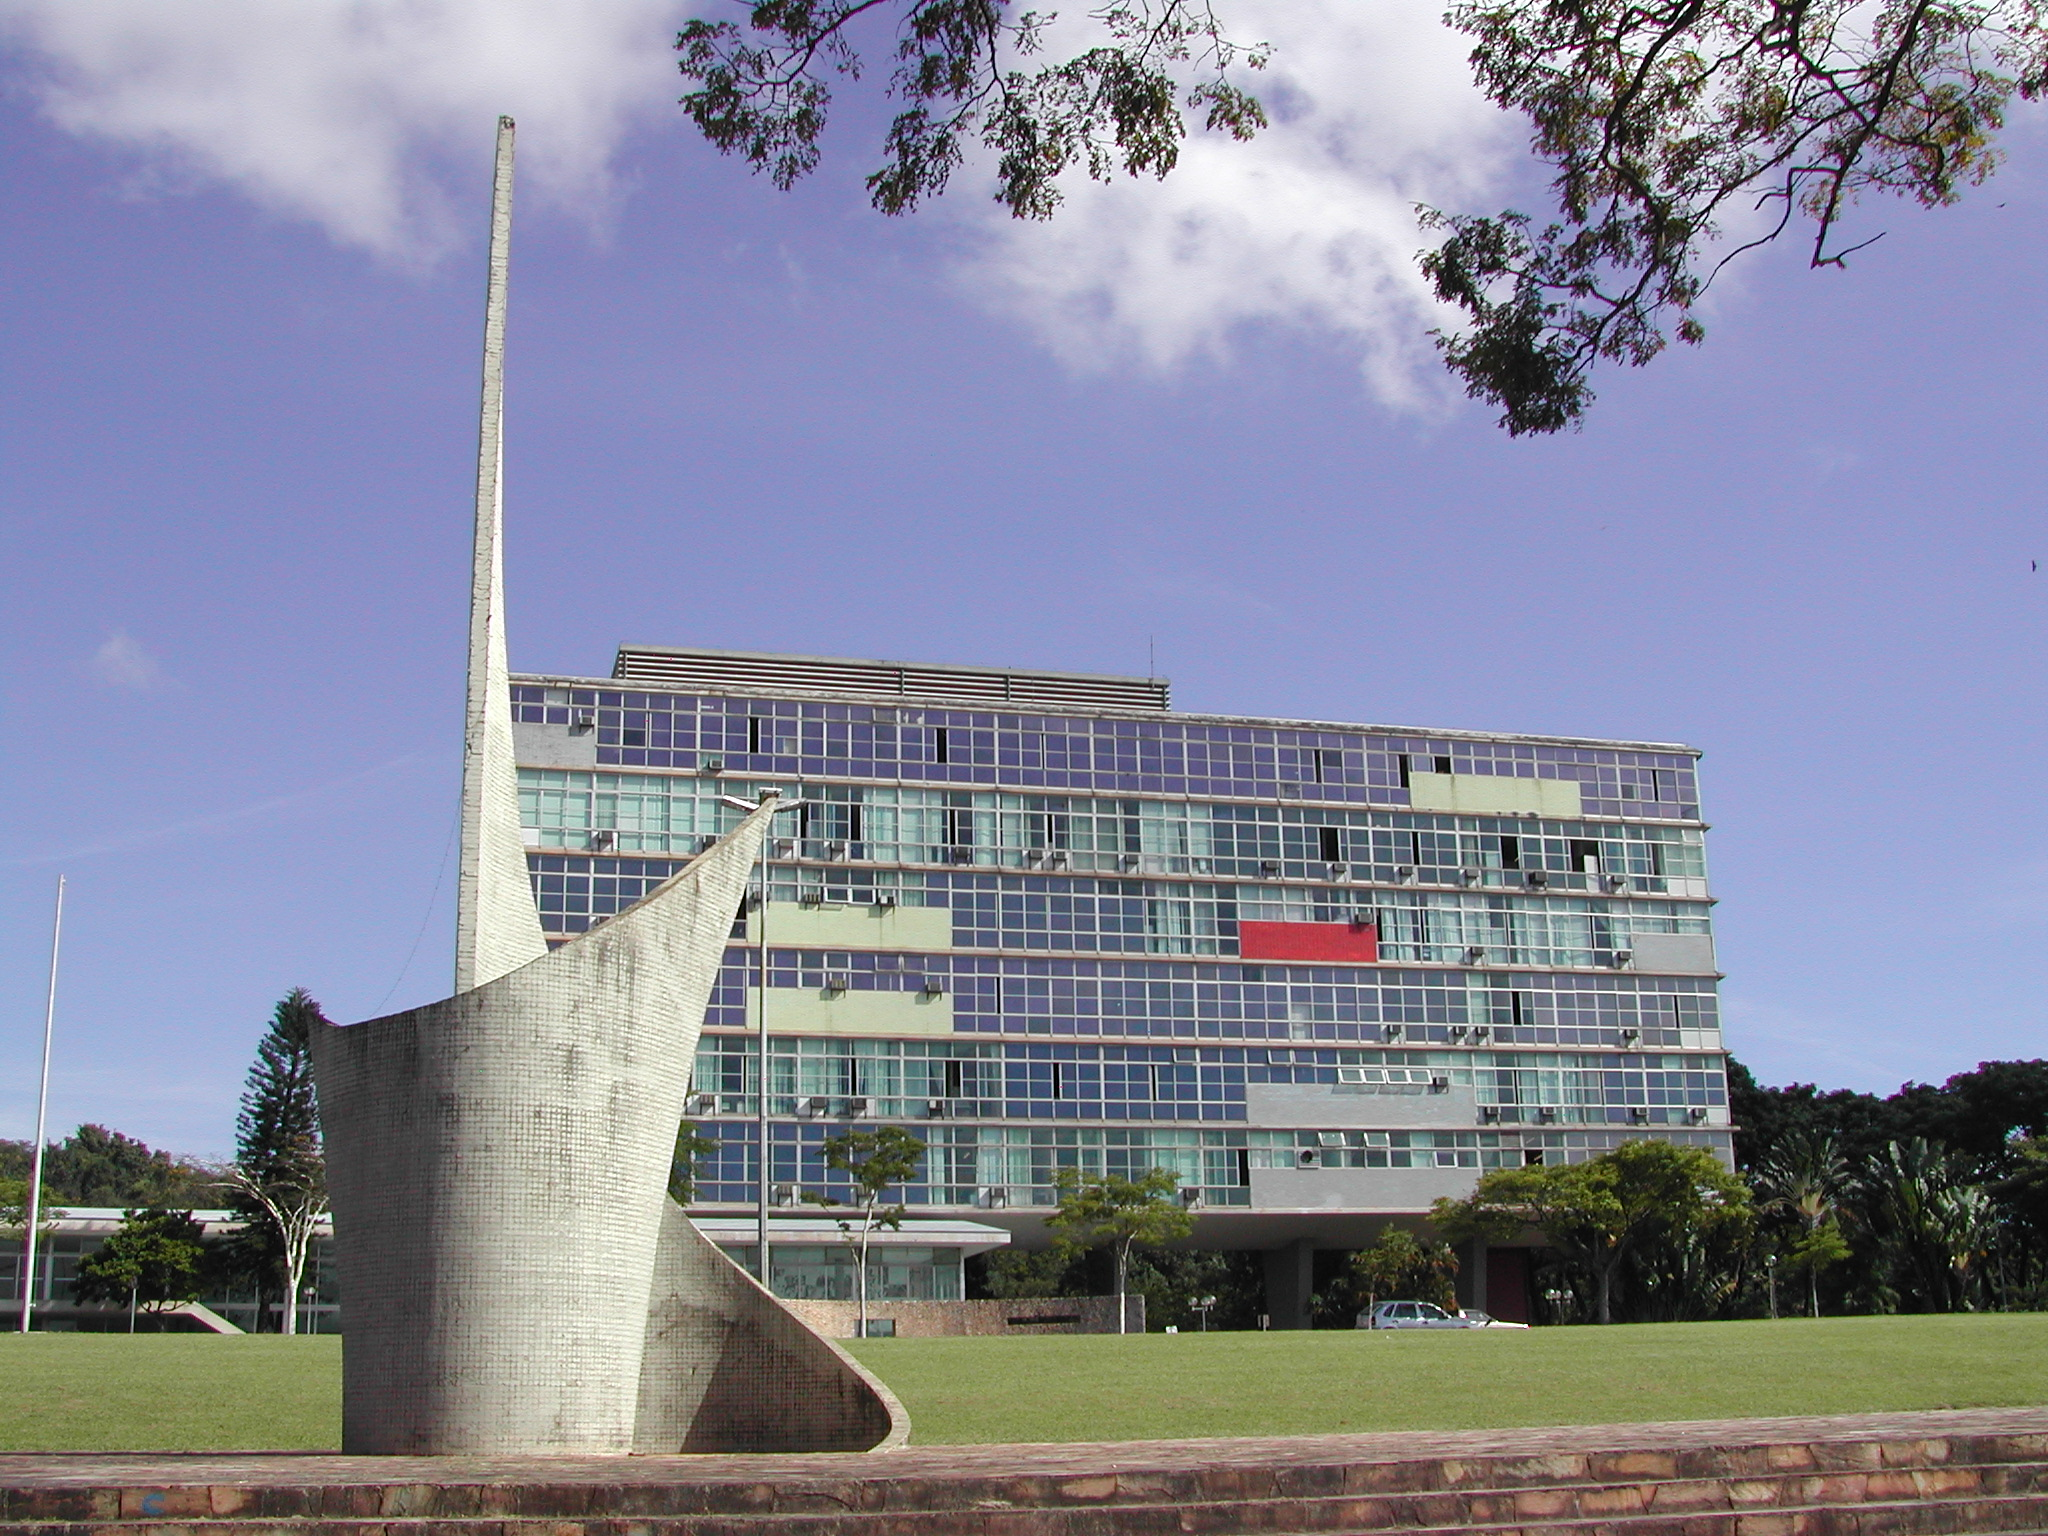
\includegraphics[scale=0.3]{imagens/exemploFigura}
        \\\small{\textbf{Fonte:} Elaborada pelo autor (fonte é opcional)}%
     \end{figure}
         
\end{frame}


\begin{frame}

    \frametitle{Slide com Tabela}
    
    \begin{table}[!htbp]
       	\centering
       	\caption{Exemplo de tabela de 2 colunas (caption é opcional)}
       	\begin{tabular}{ c | c }
       		\hline
       		\textbf{Coluna 1} & \textbf{Coluna 2} \\ \hline
       		Dado 1a           & Dado 2a           \\ \hline
       		Dado 1b           & Dado 2b           \\ \hline
       		Dado 1c           & Dado 2c           \\ \hline
       		Dado 1d           & Dado 2d           \\ \hline
       	\end{tabular}
       	\\ \vspace{0.2cm}
       	\small{\textbf{Fonte:} Elaborada pelo autor (fonte é opcional)}%
     \end{table}
         
\end{frame}


\begin{frame}

    \frametitle{Slide com Quadro}
    
    \begin{quadro}[!htbp]
       	\centering
       	\caption{Exemplo de quadro (caption é opcional)}
       	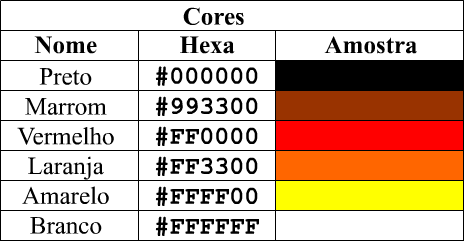
\includegraphics[scale=.3]{imagens/exemploQuadro}
        \\ \vspace{0.2cm}
       	\small{\textbf{Fonte:} Elaborada pelo autor (fonte é opcional)}%
    \end{quadro}
         
\end{frame}


\begin{frame}

    \frametitle{Slide com Equação}
    
    \begin{equation}
        \sum_{i=1}^{n} i = \frac{n(n+1)}{2}
        \label{eq:exemplo}
    \end{equation}
         
\end{frame}


\begin{frame}

    \frametitle{Slide com Código Fonte}
    
    \centering
    \resizebox{10cm}{!}{%
        \lstinputlisting[language=Java]{fontes/ClasseExemplo.java} 
    }
    
\end{frame}


\begin{frame}

    \frametitle{Slide com Lista de Itens}
    
    \begin{itemize}
       	\item \textbf{Item 1:} texto...;
       	\item \textbf{Item 2:} texto...;
       	\begin{itemize}
       		\item \textbf{Subitem:} texto...;
       		\item \textbf{Subitem:} texto...;
       		\item \textbf{Subitem:} texto...;
       	\end{itemize}
       	\item \textbf{Item 3:} texto...;
       	\item \textbf{Item n:} texto....
    \end{itemize}
         
\end{frame}


\begin{frame}

    \frametitle{Slide com Lista Numerada}
    
    \begin{enumerate}
       	\item \textbf{Item:} texto...;
       	\item \textbf{Item:} texto...;
       	\begin{enumerate}
       		\item \textbf{Subitem:} texto...;
       		\item \textbf{Subitem:} texto...;
       		\item \textbf{Subitem:} texto...;
       	\end{enumerate}
       	\item \textbf{Item:} texto...;
       	\item \textbf{Item:} texto....
    \end{enumerate}
         
\end{frame}


\begin{frame}

    \frametitle{Formatação de Texto e Referências}
    
    Todas as macros que você utilizou na elaboração do seu documento podem ser usadas nas apresentações, com exceção do ambiente verbatim. Você poderá criar citações formatadas também, mas as referências não serão geradas em um slide, apenas serão exibidas no texto. Por exemplo:
    
    \begin{itemize}
        %\item \cite{Abedi2014, Agaisse1995};
        %\item \cite{AgapitoTenfen2014, BtNomenclature2016, Nelson2014};
        %\item \citeauthorandyear{Agaisse1995};
        %\item \citeauthorandyear{Abedi2014};
        %\item \citeauthorandyear{BtNomenclature2016};
    \end{itemize}
         
\end{frame}

% não mexa!

\begin{frame}<presentation:0>
    \addtocounter{framenumber}{-1}
    \bibliography{referencias}
\end{frame}

\end{document}
